\chapter{Политика и экономика}

\section{Восемь богачей мира владеют половиной богатств Земли}
Восемь \ed{богач\'{е}й}{бог\'{а}ч}{rich person} мира владеют половиной \ed{бог\'{а}тств}{бог\'{а}тство}{wealth} Земли. Всего восемь \explain{толстосумов}{толстосум: moneybag} \explain{владеют}{владеть/завладеть: to possess (влад\'{е}ю, влад\'{е}ешь, влад\'{е}ют)} тем же состоянием, что принадлежит беднейшей половине населения Земли. К такому выводу пришли исследователи благотворительной организацией Oxfam. Более того, исследование показало, что уже в ближайшие 25 лет в мире может появиться первый триллионер. Чтобы потратить такое состояние, н\'{у}жно ежедневно в течение 27 столетий и еще 38 лет расходовать по одному миллиону.

Восемь миллиардеров владеют тем же состоянием, которое находится в руках 3 миллиардов 600 миллионов человек, отмечает РИА Новости.

Великолепную восьмерку возглавляет основатель Microsoft Билл Гейтс. Его состояние оценивается в 75 миллиардов долларов. У Амансио Ортеги 67 миллиардов. Экс-президента Inditex женщины знают по марке магазинов одежды Zara. Третью ступень пьедестала богатства занимает американский \explain{предприниматель}{business-person; entrepreneur} Уоррен Баффетт с состоянием почти 61 миллиард долларов.

Оставшаяся пятёрка толстосумов выглядит так: мексиканский бизнесмен Карлос Слим Элу --- 50 миллиардов долларов, глава компании по электронной торговле Amazon Джефф Безос --- чуть более 45 миллиардов долларов, основатель соцсети Facebook Марк Цукерберг --- чуть менее 45 миллиардов долларов, глава корпорации Oracle Ларри Эллисон с состоянием 43 миллиарда и 600 миллионов долларов и владелец агентства деловой информации Майкл Блумберг с 40 миллиардами.
В 2010 году считалось, что стоимость имущества, которым владеют половина беднейших жителей Земли, равна совокупному состоянию 43 богатейших людей планеты. Так что за последние шесть лет ситуация лишь усугубилась.

``Это возмутительно, что такие средства сосредоточены в руках всего нескольких человек, когда каждый десятый в мире вынужден выживать на менее чем два доллара в день'', --- отметил исполнительный директор Oxfam Уинни Бьянима.

По его мнению, неравенство способствует тому, что сотни миллионов человек находятся в ловушке бедности.

``Это разрушает наши общества и подрывает демократию'', --- настаивает Бьянима.

Сегодня семь из десяти человек живут в странах, где за последние три десятилетия неравенство в доходах возросло. При этом всего один процент населения планеты владеет таким же богатством, как 99 процентов тех, кто не попал в золотой процент.

Кроме того, чтобы труд женщин в мире оплачивался так же, как и мужской, понадобится еще порядка 170 лет, отмечают в Oxfam.

Oxfam (Oxford Committee for Famine Relief) основана в Оксфорде в 1942 году для помощи голодающим. Ее цель --- решение проблем бедности и связанной с ней несправедливости во всем мире. Международное объединение сейчас объединяет 17 организаций в более чем 90 странах мира.

\newpage
\section{Белорусы голосуют за новую конституцию}

\textit{Что изменится в жизни страны и ее граждан?}

\textit{Источник: \url{https://lenta.ru/articles/2022/02/27/bel_ref/}}

27 февраля в Белоруссии пройдет референдум о внесении изменений в конституцию. Согласно новой редакции основного закона, страну ждет перераспределение властных полномочий в пользу Всебелорусского народного собрания (ВНС), закрепление на конституционном уровне ценностей патриотизма и ослабление роли президента. Власти республики во главе с Александром Лукашенко называют событие историческим и говорят о больших переменах в стране в случае принятия поправок. Оппозиция относится к этим заявлениям скептически и обвиняет руководство Белоруссии в имитации политического процесса. «Лента.ру» побеседовала с белорусскими и российскими политологами о перспективах конституционной реформы и узнала, зачем руководство Белоруссии меняет основной закон, как эти перемены воспринимаются в обществе и что они означают для России.

\textbf{Нужен ли референдум белорусам?}

\textit{\textbf{Алексей Дзермант}, политолог, директор Центра изучения и развития континентальной интеграции «Северная Евразия»}

Я участвовал во многих площадках [обсуждения поправок в конституцию]. На некоторых присутствовало по тысяче человек. Скажу, что это абсолютно не протокольные мероприятия, а живые беседы — люди интересуются разными пунктами [поправок в конституцию]. Я бы сказал, что общество разогрели. Оно готово к обсуждению и активному участию. Наибольший интерес вызывает раздел новой конституции, в котором говорится о ВНС. Людей интересует новая конфигурация политической системы. Они спрашивают, не будет ли двоевластия, останется ли Белоруссия президентской республикой. На все вопросы ответа нет, должен еще быть принят отдельный закон о ВНС.

\textit{\textbf{Франтишек Вечерко}, старший советник бывшего кандидата в президенты Белоруссии Светланы Тихановской}

Интерес к референдуму среди белорусов небольшой, потому что он не решает первопричины кризиса — то, что Лукашенко отказался уходить. К референдуму многие относятся как к фарсу.

\begin{fancyquotes}
    Референдум в Белоруссии — это ритуал советского типа, где решение понятно заранее и происходит симуляция народной любви
\end{fancyquotes}

Проект конституции, который они предложили, очень плох. Там перемешаны и Великая Отечественная война, и подвиг народа, и патриотизм, и личное, и гражданское. Все это делает проект неуместным, и белорусы это видят.

\textit{\textbf{Петр Петровский}, политолог, эксперт общественного объединения «Белая Русь»}

Действующая редакция конституции имеет очень большой налет либеральных утопических взглядов. Она принималась в те годы, когда гуманитарная отрасль Белоруссии находилась под влиянием западных нарративов.

А у нас ведь ментальность не протестантская, не такая автономная, как на Западе. Многие нормы, вопросы идентичности, этики и морали у нас принято регулировать на общественных началах. И те нормы, которые на Западе относятся к частной жизни, у нас являются частью жизни общественной. Изменилось и время. На Западе в 1996 году никто не говорил про гей-браки, никто не посягал на традиционные семейные ценности.

\textit{\textbf{Дмитрий Болкунец}, белорусский политолог}

В обсуждении конституции должны принимать участие разные силы — не как сейчас, когда несколько тысяч граждан находятся в тюрьме по политическим соображениям, огромное количество людей находится в эмиграции. В таких условиях это не имеет никакого смысла.

В новой редакции конституции достаточно много популистских лозунгов. Но что бы ни было прописано в основном законе, вопрос в том, как это будет реализовано.

\begin{fancyquotes}
    На самом деле граждане Белоруссии готовы согласиться с любой конституцией — главное, чтобы Лукашенко ушел. Это первостепенная задача
\end{fancyquotes}

\textit{\textbf{Богдан Безпалько}, российский политолог, член Совета по межнациональным отношениям при президенте России}

Настроения в белорусском обществе можно охарактеризовать как апатичные. Лукашенко если и не любят, то пассивно. Протест против него считают бессмысленным — просто потому, что его задавят силой. В республике нет никакой оппозиции. Она либо выехала за границу, либо сидит очень тихо.

Часть населения республики сейчас просто пытается выжить. В Белоруссии сильно выросли цены, инфляция двузначная. Из-за санкций экономика там действительно пошатнулась. Из Минска даже многие врачи и преподаватели уехали. Кто-то уезжает на работу в Россию, кто-то в Литву, в Польшу. Людям не до конституционного референдума и протестов.

\textbf{Что референдум дает Лукашенко и белорусским элитам?}

\textit{Алексей Дзермант:} Президент хочет удержать страну от цветной революции или государственного переворота. Действующая конституция написана под конкретного человека — Александра Лукашенко. Нужно сделать ее более универсальной, чтобы она работала и с другими президентами. Прописать органы и механизмы, которые не позволили бы с государством что-то сделать. Вот это ключевой вопрос удержания страны.

Также изменения вызваны естественным развитием белорусской политической системы. Люди требуют, чтобы какие-то полномочия передавались на иные этажи власти. Общество созрело для этого. Лукашенко понимает, что часть его сверхполномочий можно отдать другим органам. Система должна демократизироваться.

\textit{Франтишек Вечерко:} Первоначально идея изменения конституции была в том, чтобы Лукашенко мог обеспечить себе безопасное место, если вдруг ему придется покинуть должность президента. Чтобы он смог, как бывший президент Казахстана Нурсултан Назарбаев, получить пост «главного уважаемого человека». Но теперь Лукашенко поменял мнение. Он озабочен тем, как бы ему день простоять и ночь продержаться. Сделать фикцию, чтобы ничего не менять.

\begin{fancyquotes}
    Очень маловероятно, что Лукашенко собирается покинуть свой пост. Транзит не начнется с этим референдумом
\end{fancyquotes}

Но новая конституция не решит кризис, она создаст для Лукашенко больше рычагов для влияния на ситуацию. То, что он предлагает в качестве конституционной реформы, может формально менять систему власти, однако по факту все будет решаться так же, как решалось раньше. Он получит должность председателя ВНС — типа генсека ЦК КПСС — и станет совмещать ее с должностью президента. Будет сам контролировать орган, который должен контролировать его.



\textit{Петр Петровский:} Главной задачей конституционной реформы является трансформация «персонального Лукашенко» в «Лукашенко коллективного». Благодаря наделению ВНС полномочиями контролировать решения президента, выбирать ЦИК и судей Верховного и Конституционного судов мы можем жестче придерживаться пути разделения властей.
Всебелорусское народное собрание в Минске, 2021 год

С 1996 года, [когда была принята действующая редакция конституции], многое изменилось. Тогда в стране было чрезвычайное положение: после распада СССР разваливались экономика и государственные институты. Теперь нам надо выстраивать новую систему, в которой будет реальное разделение властей, независимые суды и коллективное руководство.

Референдум однозначно запускает процесс транзита власти в Белоруссии. Но вопрос в том, когда этот транзит произойдет.


\begin{fancyquotes}
    Если во время протестов 2020 года Лукашенко собирался покинуть пост после принятия новой конституции, то теперь, после стабилизации ситуации, его мнение поменялось
\end{fancyquotes}

Он задал себе вопрос: нужно ли ему идти на новые выборы в 2025 году? Мое мнение — да, нужно. За пять лет нового срока ему необходимо подготовить персональную преемственность. Данный вопрос не решен до сих пор.


\textit{Дмитрий Болкунец:} Я думаю, референдум проводится для политического транзита. Но надо понимать, что Лукашенко — человек хитрый, неустойчивый и амбициозный. Он до последнего будет биться за политическое влияние.

На мой взгляд, Лукашенко уйдет [с президентского поста] и в Белоруссии состоятся очередные президентские выборы не позже, чем в России состоятся выборы президента — в марте 2024 года. Как и в какой форме это будет происходить, сказать сложно.

\textit{\textbf{Станислав Бышок}, директор международной мониторинговой организации CIS-EMO}

Некоторые говорят, что новая конституция демократизирует Белоруссию. Но ведь и в старой не написано, что оппозиционная активность запрещена, а лидером страны может быть только человек по имени Александр Лукашенко. Это все лишь попытка создать вид некой демократизации.

Такие страны, как Белоруссия, пытаются изобрести гибридный велосипед: пытаются его улучшить, но никакого содержательного аспекта в этом нет, помимо сохранения действующей власти под другим названием.

Можно сказать, что конституционный референдум запускает транзит власти в Белоруссии, чтобы его не запускать. На пике протестов Лукашенко заявлял, что, конечно же, он скоро уйдет, но сейчас говорит об этом уже с меньшей охотой.

\textit{\textbf{Евгений Минченко}, президент коммуникационного холдинга «Минченко консалтинг» }

Лукашенко проводит конституционную реформу под себя. Он не заинтересован ни в каких демократических реформах. ВНС будет органом-симулякром, который будет формироваться не путем прямых выборов, а путем фактического назначения его участников.

У Лукашенко и его команды есть вполне обоснованные сомнения в электоральной поддержке, поэтому они создают структуры, которые зависят не от воли избирателей, а от начальства. Примеры подобного рода транзитов власти мы видели у [президента Турции Реджепа Тайипа] Эрдогана и ряда других правителей — когда меняется формальная составляющая без изменений фактической системы принятия политических решений. Я думаю, что в Белоруссии будет то же самое.

\textit{Богдан Безпалько:} Задача Всебелорусского народного собрания — это концентрация власти в руках президента Лукашенко и придание ему суперстатуса, которым не обладал даже российский император Николай II в конституционный период — то есть практически статуса монарха. Он будет обладать неподсудностью и иметь сверхполномочия как президент и председатель ВНС.

В белорусской конституционной реформе интересно и то, что она обязывает кандидата в президенты обладать десятилетним стажем работы в государственных органах. И при этом на него не должно быть никакого компромата, даже анонимного. Не говоря уже о том, что кандидат должен родиться на территории независимой Белоруссии, то есть после 1991 года. Это фактическое аннулирование активного избирательного права.

\textit{\textbf{Андрей Суздальцев}, российский политолог}

[Создаваемое после принятия новой конституции] ВНС не будет являться избираемым собранием. Туда будет назначаться высшая номенклатура из разных сфер. То есть это будут представители той группировки, которая уже находится у власти. Никакого отношения к народовластию ВНС не имеет. Это остаток авторитарного режима.

ВНС ни за что не будет отвечать, но получит право влезать во все дела. Перед ним будет отчитываться премьер-министр, представители собрания смогут отменять итоги выборов, а Лукашенко, став главой президиума ВНС, сможет лишать полномочий действующего президента.

\begin{fancyquotes}
    Неограниченные полномочия сделают из этого органа почти что коллективного монарха, который при этом будет несменяемым и совершенно неподотчетным
\end{fancyquotes}

Лукашенко решил создать усиленный вариант того, что сделал [первый президент Казахстана Нурсултан] Назарбаев, когда уходил со своего поста и пожизненно подчинял себе Совет безопасности республики. Однако Назарбаева это не спасло.

Лукашенко не понимает одного: в авторитарных режимах, если ты хоть на шаг сдвинулся со своей позиции, ты уже не вернешь себе былую власть. Это и обнаружил Назарбаев, когда оказалось, что подконтрольный ему [президент Казахстана Касым-Жомарт] Токаев все равно оказался сильнее.

\textbf{Есть ли в белорусском референдуме выгода для России?}

\textit{Алексей Дзермант:} Более стабильная страна, где действует универсальный закон, заточенный не только под одного человека, для России выгодна. Чтобы было стабильное, предсказуемое государство, с руководством, которое крепко держит бразды правления.

Если по результатам референдума люди примут поправки, то они укрепят власть Лукашенко. А это значит — поддержку Кремля. Москва заинтересована прежде всего в том, чтобы в Белоруссии была сильная власть, союзная России. Лукашенко это воплощает, и конституция все это подтверждает и развивает.

\textit{Дмитрий Болкунец:} Я считаю, что Лукашенко является токсичной фигурой для Москвы. Кроме того, он абсолютно бесполезен в плане стратегического сотрудничества. Он ничего делать не будет.

В России это понимают. Косвенный пример: российский Минфин отказывается, судя по заявлениям [главы министерства финансов Антона] Силуанова, выдавать Белоруссии кредиты, которые та запрашивает. Будет выдавать только средства для реструктуризации кредитов прошлых лет. Россия не вкладывает новые деньги в Белоруссию при Лукашенко.

\textit{Петр Петровский:} Единственный внешнеполитический вопрос в новой редакции конституции связан с избавлением от рудимента о стремлении Белоруссии к нейтралитету. Эта норма сохранялась в законе с 1994 года. Но ее логично было бы убрать еще в 1995 году, когда на референдуме было принято решение о строительстве Союзного государства с Россией.

\textit{Станислав Бышок:} Многие подались заблуждению, что принятие в Белоруссии новой конституции выгодно российскому руководству, которое якобы заинтересовано в демократизации республики. Это неправда. Россия в этом не заинтересована.

\begin{fancyquotes}
    В Кремле нет людей, которые продвигали бы альтернативную Лукашенко фигуру. Но я не могу назвать ни одного человека в российской власти, который бы симпатизировал ему
\end{fancyquotes}

То есть они по миллиону причин не любят Лукашенко, но вместе с тем опасаются, что на его место может прийти коллективная Светлана Тихановская, а на границе с Россией появятся базы НАТО. В Кремле свыклись с фигурой действующего белорусского президента.

Принятие новой конституции никак не повлияет на скорость продвижения интеграции в рамках Союзного государства. Это не связанные между собой параллельные процессы.

\textit{Богдан Безпалько:} Новая белорусская конституция невыгодна российским властям. Реформа основного закона только усиливает этот дикий автократический режим, который напоминает наполеоновский. При этом для Москвы он является неподконтрольным. В Кремле не могут быть уверены в том, что будет дальше. Автократ в любой момент может поступить так, как России абсолютно невыгодно. Но другого выхода сейчас нет.

Объективно Лукашенко сейчас толкает в сторону России его дикая токсичность для Запада и то, что он там объявлен нерукопожатным достаточно давно. Но в случае каких-либо изменений Лукашенко точно так же может побежать от России. И мы знаем, что на Западе достаточно циничные люди, чтобы не обращать внимание на то, что он «последний диктатор Европы».

\textbf{Как референдум повлияет на отношения Белоруссии с Западом?}

\textit{Алексей Дзермант:} Вряд ли после референдума будет хуже. Насколько я знаю, уже были заявления о непризнании любых итогов голосования. Новая конституция все равно сделает позицию власти легитимной. Игнорировать итоги голосования не сможет никто, даже Европа. Если народ проголосует за конституцию — это значит, что, хочешь или не хочешь, придется иметь дело с этой властью. Новая конституция поставит определенные точки в кризисе 2020 года.

Я не думаю, что референдум вызовет очередную волну санкций. У оппозиции нет уже той инфраструктуры для информационного давления, чтобы сообщения о якобы фальсификациях сделать массовыми. Эта инфраструктура разгромлена. Конечно, они будут пытаться. Но в целом, я думаю, результаты референдума де-факто будут признаны+ и белорусская власть будет считаться субъектом, с которым нужно вести хоть какие-то переговоры.

\textit{Франтишек Вечерко:} Уже сейчас многие депутаты из Европарламента заявили, что не признают референдум. В ОБСЕ сказали, что даже не будут посылать официальных наблюдателей. Конечно, санкции сейчас рассматриваются.

\begin{fancyquotes}
    ЕС будет вводить санкции, пока Лукашенко будет творить глупости
\end{fancyquotes}

При этом внешняя политика Минска тоже не поменяется после референдума. Думаю, что переход к ВНС ответственности за внешнеполитический курс никак на нее не повлияет. Пока Лукашенко остается наверху, все переговоры будут вестись только с ним.

\textit{Петр Петровский:} С точки зрения Запада проведение референдума тихо и гладко будет легитимировать Александра Лукашенко. Мы знаем, что уже сейчас началась активность западных партнеров по налаживанию дипломатических каналов. Были звонки представителей Госдепа США [министру иностранных дел Белоруссии Владимиру] Макею, контакты руководителей Генштабов США и Белоруссии — это то, что уже было. Я считаю, что Запад после референдума будет дальше инициировать оживление контактов.

Их задача — снова восстановить иностранных агентов в Белоруссии, чтобы не дать развиваться евразийским интеграционным процессам в стране. Они не идиоты, они понимают, что время [оппозиционного политика Светланы] Тихановской проходит. Теперь нужны новые инструменты влияния и лоббирования изменений и реформ в республике.

\textit{Дмитрий Болкунец:} Белорусские власти будут пытаться торговаться с Западом, если референдум пройдет благополучно и спокойно. Будут пытаться продавать Лукашенко в Европе как надежного политика, с которым все в Белоруссии смирились. Я думаю, это не получится, потому что на Западе есть консенсус, что с Лукашенко работать не имеет никого смысла.

\textit{Станислав Бышок:} Принятие новой конституции никак не повлияет на отношения Белоруссии с европейскими странами. На Западе референдум никто не признает. Он никого не впечатлит, за этим не последует нового витка санкций. Это скорее внутренняя история.

\textit{Богдан Безпалько:} Конечно, на Западе не будут признавать этот референдум, однако по большому счету ему большого значения не придают. Особенно после президентских выборов 2020 года. Все понимают, что Лукашенко, подавив протесты, полностью контролирует свою страну и будет делать все, что захочет.

Референдум добавит лишний штрих в картину, но принципиально ничего не изменит. Могут быть какие-то санкции, но вряд ли они будут порождены именно конституционной реформой. И пока Лукашенко может опираться на Россию в экономическом и военном отношении, подобные меры не будут иметь решающего эффекта.

\textbf{Возможны ли новые протесты в Белоруссии по итогам референдума?}

\textit{Петр Петровский:} Белорусская оппозиция уже пытается запугать членов ЦИК, дестабилизировать работу государственных органов через попытки минирования, взлома электронных систем. Они занимаются теми процессами, на которые могут повлиять.

Внутри страны вряд ли имеется какой-то протестный потенциал. Во-первых, общество устало от излишней политизации. Во-вторых, государство задерживало и привлекало к ответственности всех участников незаконных протестов, государство ужесточило наказания. Эти факторы по сарафанному радио разносятся среди населения и его протестная активность резко падает. Я сегодня не вижу готовых даже попытаться подать заявку на массовое мероприятие.

\textit{Станислав Бышок:} В Белоруссии отсутствуют предпосылки для массовых протестов после референдума, как это было в 2020 году. Для революции нужен революционный класс, какие-то активные лидеры и раскол внутри политических элит. Видных представителей оппозиции в республике либо посадили в тюрьму, либо выдавили из страны. Элитный раскол так и не случился.

\begin{fancyquotes}
    В 2020 году никто не протестовал против конституции, никто не требовал проведения референдума по ней. Это был протест против Лукашенко. Теперь народу предлагается новая конституция, которая сохраняет у власти этого человека. Это издевательство
\end{fancyquotes}

\textit{Евгений Минченко:} В Белоруссии на сегодняшний день разгромлена протестная инфраструктура. У оппозиции нет организационных или информационных возможностей, чтобы устроить масштабную агитацию против новой Конституции. Невелика и вероятность массовых протестов. Они уже были, и их достаточно жестко подавили.

Ранее российские власти говорили о том, что власти Белоруссии должны наладить диалог с оппозицией и оппозиционными слоями населения. Однако мы видим, что сегодня этого не происходит, а диалоговые форматы носят имитационный характер.

\textit{Дмитрий Болкунец:} Я не ожидаю, что после протестов состоятся масштабные выступления. Во-первых, референдум мало что решает, во-вторых, выступления явно будут гаситься властями. Часть граждан пойдут на участки, кто-то поддержит призывы оппозиционных политиков портить бюллетени, могут быть отдельные выступления.

Я бы обратил внимание на акции в городах Европы и США. Я убежден, что митинги против референдума будут у посольств и консульств Белоруссии. Это можно считать продвижением оппозиционной повестки.

\textit{Андрей Суздальцев:} Не стоит ждать каких-либо протестов после референдума. Белорусская оппозиция обескровлена. Ее лидеры либо находятся в тюрьмах, либо выехали за рубеж. Конечно, они мечтают, чтобы референдум стал толчком к народным выступлениям. Но подобные мероприятия надо готовить, вкладывать в них деньги. Ничего этого сделано не было.

Рассчитывать на народную инициативу здесь тоже сложно, потому что люди очень разочарованы августом-октябрем 2020 года. Люди поняли, что ходить с шариками и сердечками против авторитарного режима — это все равно что бросаться на амбразуру.

\newpage
\section{НДФЛ без границ}
\textit{Надолго уехавшим из России выпишут 13-процентный налог}

{\it Источник: \url{https://www.kommersant.ru/doc/5988499}}

Минфин доработал поправки о новых правилах уплаты НДФЛ гражданами, более полугода работающими из-за рубежа на российские компании. Согласно обновленной версии, доходы, полученные как по трудовым договорам, так и по договорам гражданско-правового характера, с 2024 года будут облагаться по стандартной ставке 13\%. Таким образом, одинаковый налог будет взиматься как со штатных работников, так и с фрилансеров, как с резидентов, так и с нерезидентов. Для последних это может означать возникновение двойного налогообложения — в РФ и в новой стране пребывания. Попытаться решить проблему можно будет с помощью соглашений об избежании двойного налогообложения, перспективы практического применения которых в нынешних условиях не ясны.

Проект точечных изменений в Налоговом кодексе, предусматривающий в том числе новые правила налогообложения граждан, работающих на российские компании из-за рубежа, доработан для повторного внесения в Госдуму, сообщил в четверг Минфин. Напомним, законопроект был внесен правительством в нижнюю палату 24 апреля, но уже на следующий же день был отозван для «технических уточнений».

Изменения в части НДФЛ для уехавших, однако, оказались весьма существенными. В апрельской версии предлагалось отнести к доходам от источника в России оплату труда, полученную от российского заказчика фрилансерами, работающими по договорам гражданско-правового характера. Пока такие доходы НДФЛ в случае утраты работником резидентства, то есть после полугода проживания за рубежом, вообще не облагаются — и по прежней редакции такие физлица могли подпасть сразу под 30\% налог.

\begin{fancyquotes}
    В новой версии налог для нерезидентов также возникает — но по стандартным ставкам 13\% или 15\% (с доходов, превышающих 5 млн руб. в год).
\end{fancyquotes}

При этом к доходам от источника в России законопроект теперь относит и вознаграждения, полученные при выполнении дистанционным работником трудовой функции по договору с работодателем, являющимся российской организацией или обособленным подразделением иностранной организации, зарегистрированным в РФ,— проще говоря, налог будет взиматься как со штатных работников, так и с фрилансеров, как с резидентов, так и с нерезидентов.

Замминистра финансов Алексей Сазанов такую унификацию объясняет тем, что сейчас российским организациям как налоговым агентам приходится определять ставку налога с дохода работника в зависимости от конкретной ситуации — и «когда сотрудник работает в удаленном форме, конечно, компаниям сложно проверять, является он российским налоговым резидентом или нет». По его словам, новшество должно существенно упростить администрирование для налоговых агентов.

\begin{fancyquotes}
    Компаниям изменения, может, жизнь и облегчат, но самим нерезидентам грозят двойным налогообложением — ведь налоговые органы иностранного государства, как правило, также будут претендовать на обложение доходов своего нового резидента.
\end{fancyquotes}

Как отмечает партнер Kept Донат Подниек, для тех, кто работает в стране, с которой у РФ действует соглашение об избежании двойного налогообложения (это около 80 государств), и платит там налоги с полученной от российского работодателя зарплаты, есть возможность зачесть в РФ иностранный налог. «Правда, в течение какого-то времени, пока не вернут НДФЛ, удержанный в РФ, работник фактически уплатит налоги и в РФ, и за рубежом»,— говорит эксперт.

Как уточнил Алексей Сазанов, в случае приостановки соглашений (такая возможность сейчас обсуждается в отношении недружественных стран — см. “Ъ” от 15 марта), нормы, позволяющие зачесть уплаченный налог, продолжат действовать. Вопрос, отметим, в том, будет ли в нынешних условиях это возможным на практике при нынешнем уровне информационного обмена и сотрудничества с недружественными юрисдикциями. В самой же невыгодной ситуации окажутся те, кто уехал в страны, с которым таких соглашений нет или они денонсированы (например, с Нидерландами),— тогда доход, предупреждает руководитель практики «Структурный и налоговый консалтинг» юркомпании «Лемчик, Крупский и партнеры» Людмила Круглова, будет облагаться налогом и в России, и в стране пребывания без возможности зачета.

\begin{fancyquotes}
    Донат Подниек отмечает, что для тех, у кого должным образом оформлена работа за рубежом и российский работодатель НДФЛ не удерживает, изменения ухудшат положение работников.
\end{fancyquotes}

Но есть случаи, когда допсоглашений о дистанционной работе за рубежом нет и работодатель «для подстраховки» удерживает НДФЛ по ставке 30\% — в таком случае нагрузка снизится. Людмила Круглова отмечает, что в силу отсутствия у налоговых органов возможности автоматически проверять статус резидентства граждан, видимо, власти пришли к выводу, «что ужесточение правил не позволит собрать с уехавших граждан 30\% НДФЛ: добровольно в массовом порядке о потере статуса резидента граждане уведомлять не будут, а проверять этот статус у миллионов работников в ручном режиме невозможно».

По словам ассоциированного партнера МЭФ Legal Анны Зеленской, изменения логичны в связи с цифровой трансформацией рынка труда и распространенностью дистанционной работы. «Тезис о том, что работодатели должны следить за физическим местоположением сотрудника, наверное, действительно несколько устарел»,— говорит она.

\newpage
\section{20 лет Владимира Путина: трансформация режима}

\textit{Политолог Кирилл Рогов открывает цикл статей о том, как изменилась страна за путинские годы}

\textit{Источник: \url{www.vedomosti.ru/opinion/articles/2019/08/07/808337-20-let-putina}}

\textit{Кирилл Рогов }

20 лет назад Владимир Путин внезапно появился на политическом олимпе в образе эффективного бюрократа с силовым бэкграундом, рыночно ориентированного государственника и прагматика, чуждого идеологических пафосов. Сегодня Путин выглядит сильным авторитарным лидером (типаж «стронгмен»), увлеченным геополитическим противостоянием с Западом и идейной борьбой с мировым либерализмом, решительно жертвующим ради этого прагматическими целями развития страны. И даже когда он заговаривает о модернизации, разговор довольно быстро сбивается на виды вооружений.

\textbf{Две эпохи}



Если бы Путин ушел в 2008 г., то остался бы в истории как один из самых успешных лидеров России. После 15 лет кризисов и пертурбаций в стране наступила относительная стабилизация на условиях «управляемой демократии» (что бы это ни значило), но главное – начался период интенсивного экономического роста (7% в год в среднем) и еще более впечатляющий рост душевых доходов.

Конечно, недоброжелатели говорили бы, что причина успехов – это восстановительная фаза трансформационного цикла и рост цен на нефть. И, разумеется, в шкафах этого успешного правления уже к тому моменту скопилось немало скелетов: вторая чеченская война и ее последствия, дело ЮКОСа, создание правовых и хозяйственных гибридов в виде госкорпораций и еще кое-что. Но все это не смогло бы в исторической памяти перевесить той атмосферы успеха, на волне которой Путин покинул бы свой пост.

Вторая часть путинского двадцатилетия (2009–2019 гг.) была в значительной мере противоположна первой. Два экономических кризиса, связанных с волатильностью цен на нефть (2009 и 2015 гг.); политический кризис, вызванный московскими протестами 2011–2012 гг. и развернувший режим в сторону авторитарного ужесточения, доминирования силовых элит и их логик при принятии решений. Это последнее обстоятельство создало спусковой механизм следующего кризиса – внешнеполитического, связанного с аннексией Крыма и войной на Восточной Украине. Принятые тогда решения не были вынужденными и единственно возможными. Но эти решения, сделавшие конфронтацию с Западом основной рамкой жизни страны, окончательно закрепляли доминирование силовых элит и силовых логик во всех сферах государственной жизни.

Итак, череда экономических, внутри- и внешнеполитических кризисов (2008–2009, 2011–2012, 2014–2015 гг.), а также три войны (Грузия, Украина и Сирия) формируют основную сюжетную канву второй части путинского правления. При этом среднегодовые темпы роста упали до 0,6\% в год. В итоге в 2000 г. ВВП на душу населения в России составлял 14,5\% от уровня США и 21,5\% от уровня стран ЕС, в 2008 г. это было соответственно 22,5 и 32\%, а в 2018 г. – 21,5 и 31\%. Это и есть стагнация – неспособность сокращать разрыв с лидерами (при том что среднегодовая цена на нефть в первом периоде составила \$54 за баррель, а во втором – \$74).

\textbf{Тотальный ревизионизм}



Путин не просто не ушел в 2008 г. На самом деле в моменте неухода решительно менялось его целеполагание. В 2000 г. он пришел со сверхзадачей стабилизации и деполитизированной модернизации, выполнения которой и добивался теми способами, которые были ему в силу его компетенций доступны. Во втором периоде его сверхзадачей стало пересоздание той государственно-политической системы (несомненно, весьма лабильной и гибридной), которая складывалась по итогам первого постсоветского десятилетия.

С этим связан тотальный путинский ревизионизм второго периода: абсолютизация понятия «суверенитет», поиски новых опор в виде «скреп» и «традиционных ценностей», вытесняющих императивы модернизации, конструирование «национально ориентированных элит», фактический отказ от признания границ, сложившихся по итогам распада СССР, и решительный разворот от сотрудничества к конфронтации в отношениях с Западом.

Возможно, все это имело бы больший успех, если бы формирующаяся путинская система демонстрировала экономическую эффективность хотя бы в той мере, в какой это удавалось авторитарному Казахстану (ВВП на душу населения там в 2000 г. составлял 10\% от американского, в 2008 г. – 18\%, а в 2018 г. – 20,5\%, почти сравнявшись с российским). Но она этого сделать не смогла. И даже ее некоторые успехи в построении «эффективного авторитаризма» в отдельных сферах госуправления не могут компенсировать этого фундаментального факта.

В итоге новое целеполагание превращается в голую проповедь антилиберализма и антизападничества, переосмысление «границ русского мира» – в формирование пояса конфронтации и недоверия вокруг России, а конструирование «национально ориентированных элит» – в безраздельное господство силовиков и силовых олигархий, постоянно требующих льгот, преференций и денежных вливаний.

\textbf{Откуда и куда}



Эволюция политического режима постсоветской России может быть описана в терминах сравнительной политологии следующим образом. Режим, сложившийся к концу первого постсоветского десятилетия, можно охарактеризовать как конкурентную олигархию. Это режим, сочетающий достаточно высокую конкурентность в публичной сфере с одной стороны, и слабый, коррумпированный правопорядок – с другой. Такие режимы и сейчас существуют на Украине, в Молдавии, Киргизии и ряде стран Латинской Америки.

Путинская стабилизация 2000-х гг. и экономический рост, сопряженный с быстрым ростом рентных доходов казны, сформировали в России тип режима, который обычно называют «конкурентным авторитаризмом». В таком режиме правящая коалиция резко ограничивает возможности политической конкуренции, свободу СМИ, опираясь в том числе на достаточно широкую, но пассивную поддержку «снизу», которая (в свою очередь) обеспечена убедительной экономической динамикой. При том что правящая коалиция надежно держит власть в руках (используя в том числе административные рычаги и фальсификации на выборах), оппозиция здесь вполне легитимна, располагает определенной инфраструктурой и поддержкой граждан и элитных групп.

Авторитарный лидер или правящая партия обычно получают на выборах результат в диапазоне 60–70\%, который и демонстрирует, что примерно треть населения голосует против режима, но такое поведение считается легитимным и не угрожает его стабильности. И самое важное – эти режимы низкорепрессивные. За исключением отдельных случаев, им достаточно административных мер, чтобы секьюритизировать свое доминирование.

Такой режим существовал в путинской России примерно с 2003 по 2012 г. Политический кризис 2011–2012 гг. обозначил его закат. Однако важно подчеркнуть, что не выступления оппозиции привели к этому, а скорее экономический кризис 2008–2009 гг., подорвавший доверие граждан к режиму, что и проявилось в их реакции на фальсификацию результатов парламентских выборов в 2011 г. (в 2008 г. соизмеримые фальсификации не вызывали ни малейшего возмущения).

\begin{wrapfigure}{r}{0.7\textwidth}
    \begin{center}
        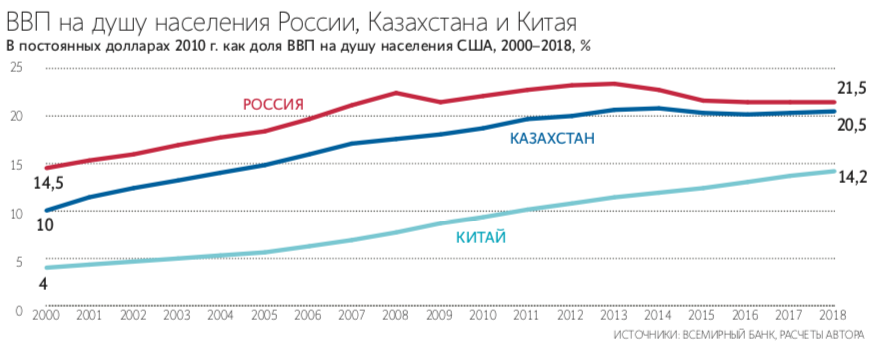
\includegraphics[width=0.68\textwidth]{img/1tbz.png}
    \end{center}
\end{wrapfigure}
\textbf{Авторитарный дедлок.} Более жесткие деспотические режимы политологи называют «авторитарной гегемонией». На выборах здесь авторитарный лидер или правящая партия регулярно получают от 75 до 99\% голосов. Что, однако, свидетельствует не об их популярности, а о том, что они оказывают гораздо более систематическое давление на оппозицию, независимые СМИ и нелояльные элитные группы, т. е. отличаются от предыдущего типа резко возрастающим уровнем репрессивности. Встречаются они сегодня почти исключительно в Азии, Африке и бывшем СССР.

Как показывает опыт ряда азиатских стран, эволюция режима от первого типа ко второму часто происходит на фоне ухудшения экономической динамики. По мере того как экономика играет все меньшую роль в обеспечении легитимности и устойчивости режима, все большую роль начинают играть две другие опоры: репрессии и идеология. В информационной политике режим переходит от фильтрации и ограничения информации к агрессивной пропаганде. Начинаются систематические преследования гражданского активизма, появляются нормы, позволяющие в уголовном порядке преследовать за слова, криминализуется уличная активность граждан.

Именно переход от режима конкурентного авторитаризма к авторитарной гегемонии составил политическое содержание последнего путинского периода – с 2013 по 2019 г. А геополитическая конфронтация выступила в качестве той идеологической рамки, которая легитимирует возрастающую репрессивность.

Хотя Россия выглядит сегодня гораздо более авторитарной страной, чем в 2012 г., этот переход, видимо, следует считать пока незавершенным. Наверное, играют свою роль развитая социальная инфраструктура мегаполисов, уровень европеизированности элит, глубина проникновения интернета и социальных медиа. Ну, и разумеется, экономический застой. Несмотря на это, Путин вряд ли оставит свои усилия по девестернизации России. И это бесплодное (в исторической перспективе) перетягивание каната скорее всего останется главным сюжетом финальной фазы его политической карьеры.




